\documentclass[../main.tex]{subfiles}
\graphicspath{{\subfix{../figures/}}}

\begin{document}
\chapter{PGP 软件应用实验}
\section{实验介绍}
PGP 软件是一款优秀的个人安全防护软件。请安装并使用该软件的主要功能,
进行相关实验,验证 PGP 软件的可用性和有效性。
%
\section{实验内容}
密钥对的产生、公钥的导出导入、文件的加密、Email 的加密和签名、文件
的粉碎、虚拟磁盘加密、磁盘空间的粉碎等功能。
%
\section{报告内容}
按功能模块进行实验,并组织书写实验步骤与实验结果,
分别以不同小节给出。实验中请使用与学号、姓名等特征信息相关的实验数据,
体现相关实验是自己所完成的。
% 具体书写建议:每个部分先给出功能性简介描述;再针对每个功能模块进行实验操作,
% 给出相关步骤的文字描述,并附上相应步骤和结果贴图。贴图要大小合适,截图清晰。
% 建议按照以下几个部分书写,不能完成的部分就删除。
% 相关的技术原理等可以适当进行一些描述,以流程图、文字结合方式为佳。
\section{PGP 密钥对的产生与管理}
% 该部分包括个人密钥对的生成、公钥的导出与导入等。
\textbf{相关技术原理}: \\
密钥是加密运算和解密运算的关键,也是密码系统的关键。密码系统的安全取决于密
钥的安全,而不是密钥算法或保密装置本身的安全。密码体制可以公开,密码设备可以丢
失,同一型号的加密设备可以继续使用,但若密钥一旦丢失或出错,就会使非法用户窃取
信息。因此密钥管理在计算机的安全保密系统中尤为重要。

生成名为``102102145''的个人密钥对.
\begin{figure}[H]
  \begin{center}
    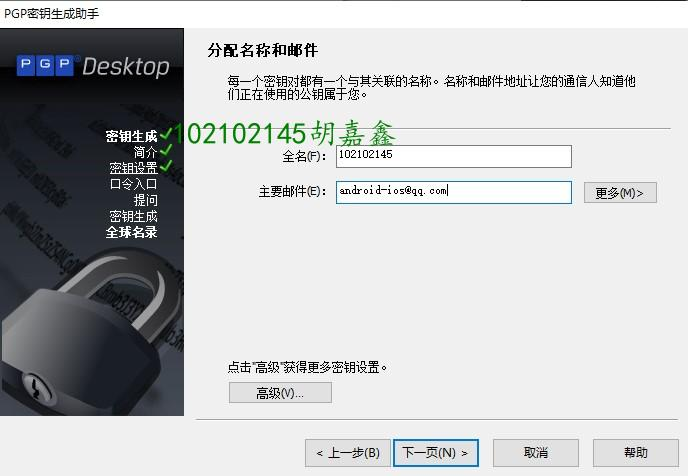
\includegraphics[width=0.45\textwidth]{1_1.jpg}
  \end{center}
\end{figure}
\begin{figure}[H]
  \begin{center}
    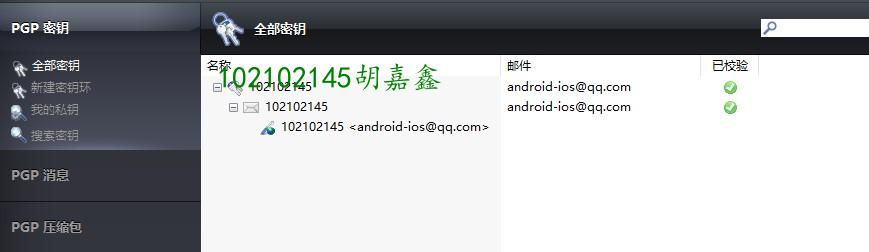
\includegraphics[width=0.45\textwidth]{1_2.jpg}
  \end{center}
\end{figure}

同理,再生成名为``hjx''的个人密钥对.
\begin{figure}[H]
  \begin{center}
    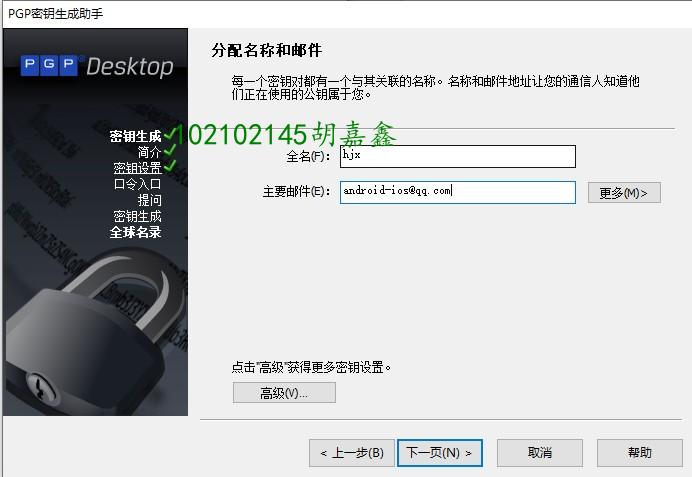
\includegraphics[width=0.45\textwidth]{1_3.jpg}
  \end{center}
\end{figure}
\begin{figure}[H]
  \begin{center}
    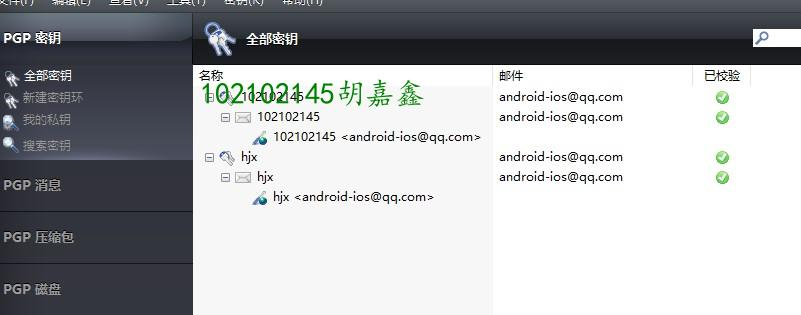
\includegraphics[width=0.45\textwidth]{1_4.jpg}
  \end{center}
\end{figure}

导出的两个公钥文件.
\begin{figure}[H]
  \begin{center}
    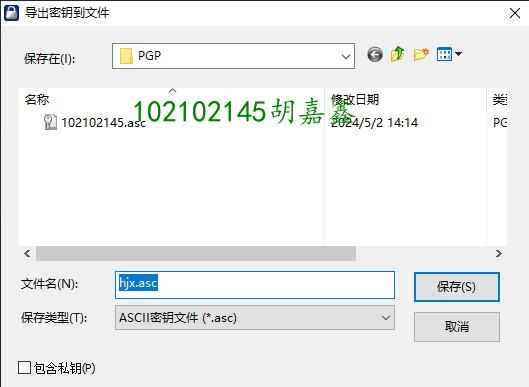
\includegraphics[width=0.45\textwidth]{1_5.jpg}
  \end{center}
\end{figure}
\begin{figure}[H]
  \begin{center}
    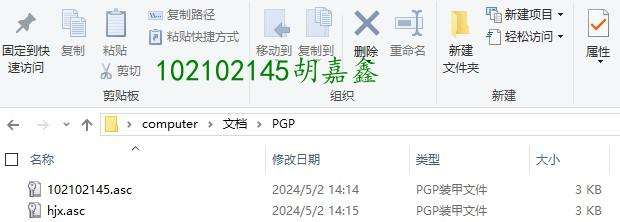
\includegraphics[width=0.45\textwidth]{1_6.jpg}
  \end{center}
\end{figure}

公钥的导入.
\begin{figure}[H]
  \begin{center}
    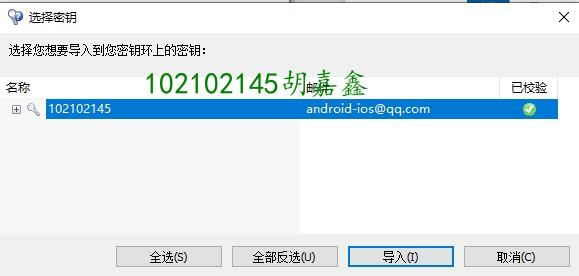
\includegraphics[width=0.45\textwidth]{1_7.jpg}
  \end{center}
\end{figure}

备份 PGPkeys 中已有密钥信息.
\begin{figure}[H]
  \begin{center}
    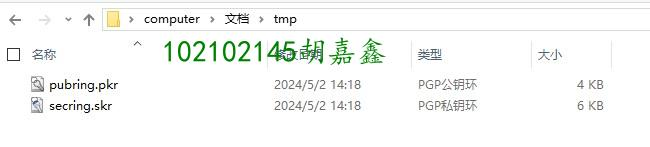
\includegraphics[width=0.45\textwidth]{1_8.jpg}
  \end{center}
\end{figure}
%
\section{文件的加密与签名}
% 该部分包括使用 PGP 对文件、文件夹的加密、加密\&签名、签名等功能的操作。
\textbf{相关技术原理}: \\
简单来说,在加密的应用场景下,发送方是用接收方的公钥加密,接收方用私钥解密。
而签名则是发送方用私钥加密,接收方用发送方公钥解密认证。

\begin{figure}[H]
  \begin{center}
    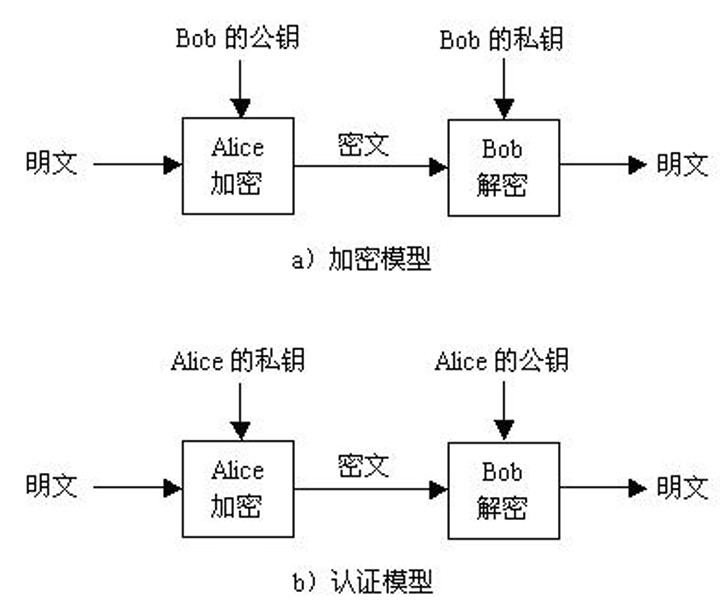
\includegraphics[width=0.45\textwidth]{1_23.jpg}
  \end{center}
\end{figure}

创建待加密文件.
\begin{figure}[H]
  \begin{center}
    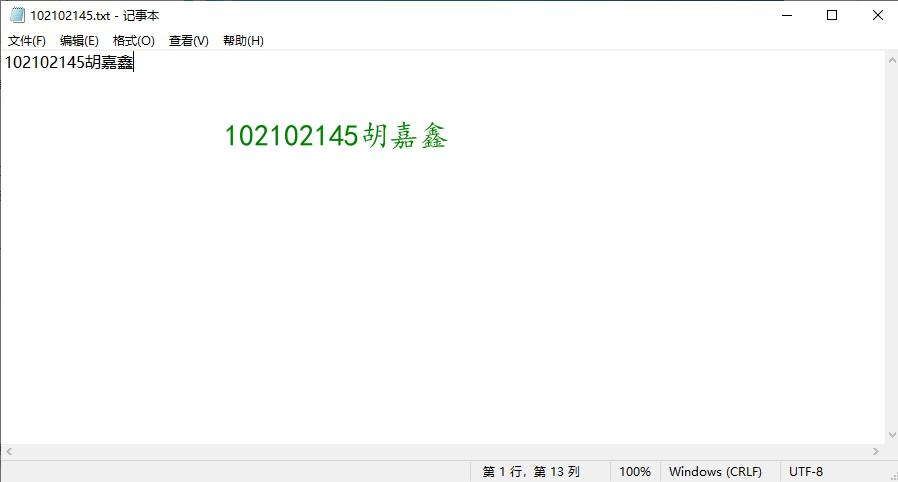
\includegraphics[width=0.45\textwidth]{1_9.jpg}
  \end{center}
\end{figure}

设置对其进行密钥保护.
\begin{figure}[H]
  \begin{center}
    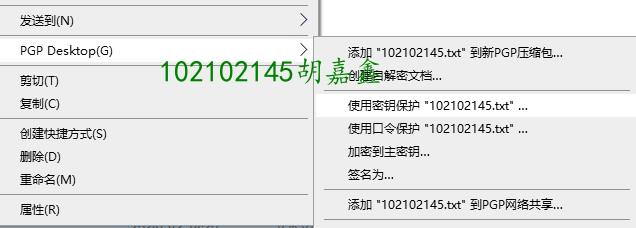
\includegraphics[width=0.45\textwidth]{1_10.jpg}
  \end{center}
\end{figure}
\begin{figure}[H]
  \begin{center}
    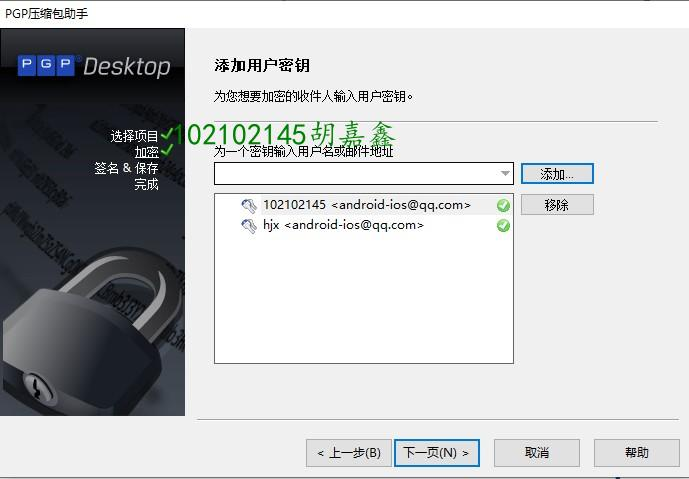
\includegraphics[width=0.45\textwidth]{1_11.jpg}
  \end{center}
\end{figure}
\begin{figure}[H]
  \begin{center}
    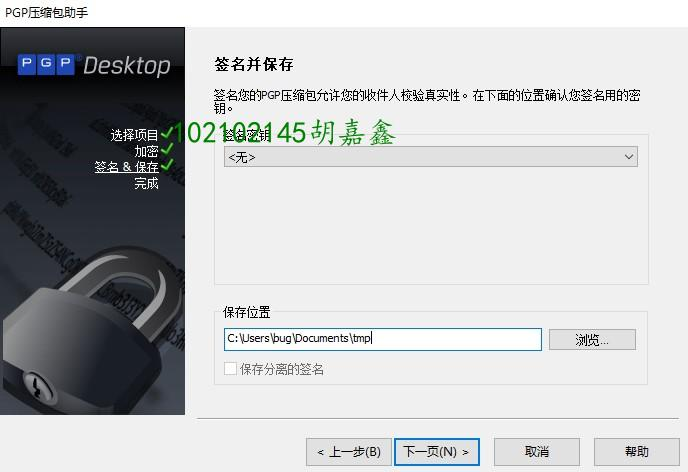
\includegraphics[width=0.45\textwidth]{1_12.jpg}
  \end{center}
\end{figure}

解密被加密文件.
\begin{figure}[H]
  \begin{center}
    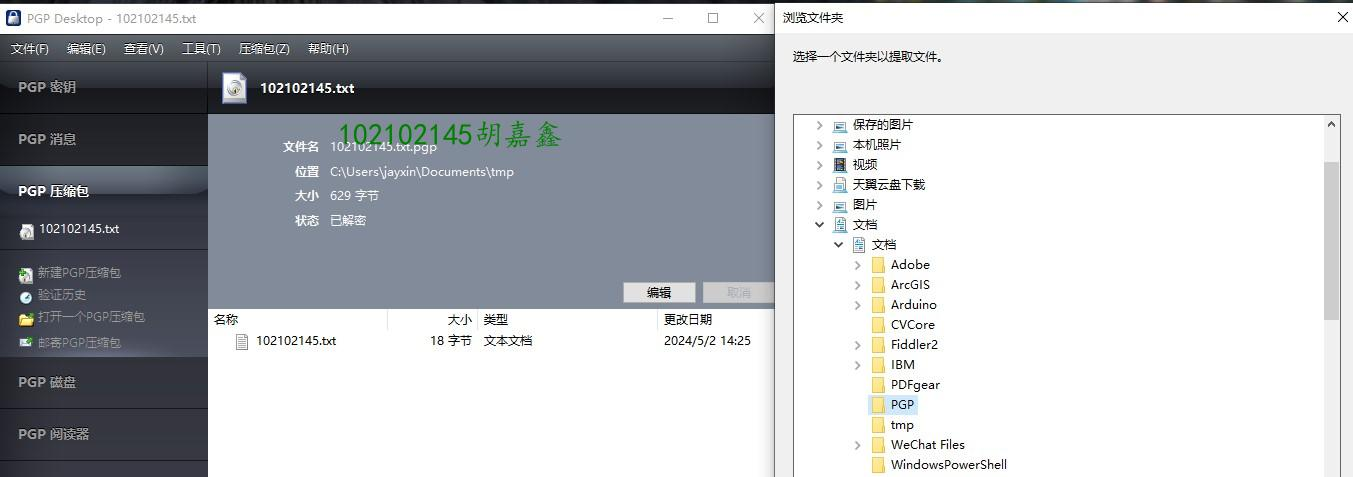
\includegraphics[width=0.45\textwidth]{1_13.jpg}
  \end{center}
\end{figure}
\begin{figure}[H]
  \begin{center}
    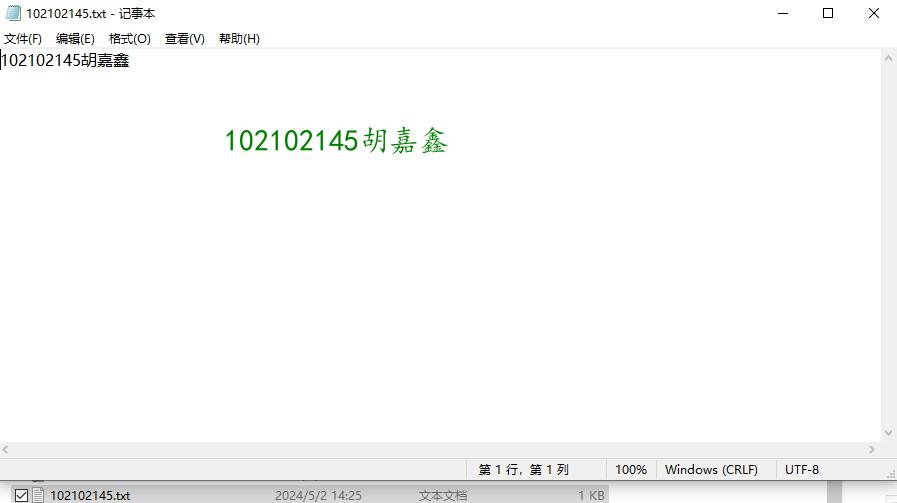
\includegraphics[width=0.45\textwidth]{1_14.jpg}
  \end{center}
\end{figure}

文件加密\&签名.
\begin{figure}[H]
  \begin{center}
    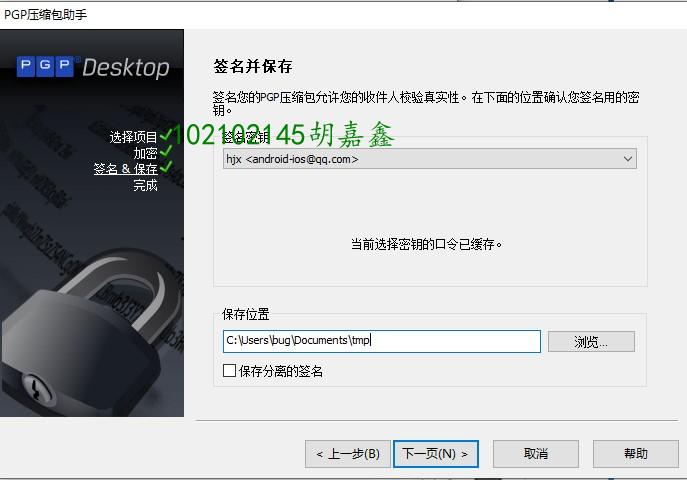
\includegraphics[width=0.45\textwidth]{1_15.jpg}
  \end{center}
\end{figure}

文件解密及其校验.
\begin{figure}[H]
  \begin{center}
    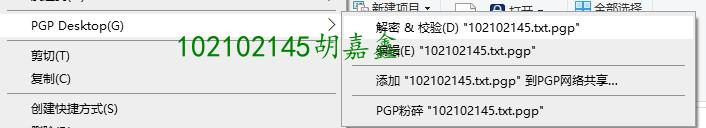
\includegraphics[width=0.45\textwidth]{1_16.jpg}
  \end{center}
\end{figure}
\begin{figure}[H]
  \begin{center}
    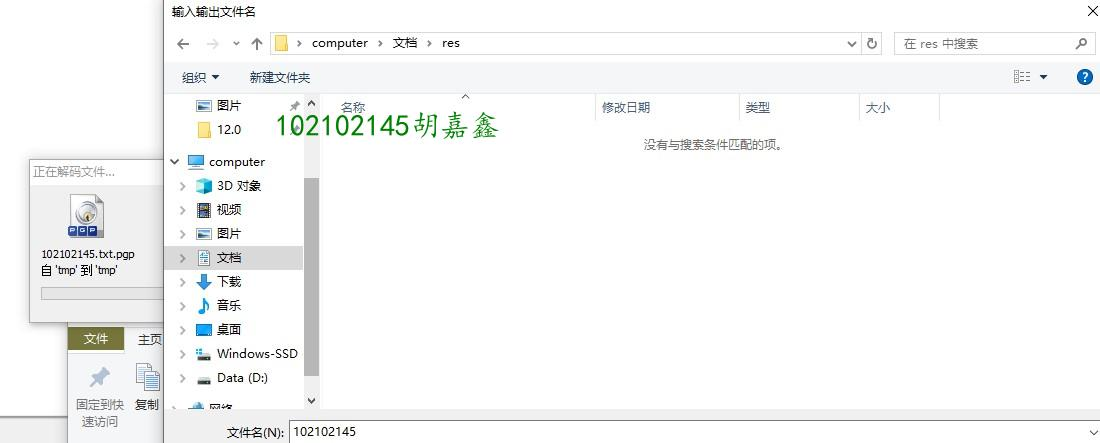
\includegraphics[width=0.45\textwidth]{1_17.jpg}
  \end{center}
\end{figure}

校验结果如下:
\begin{figure}[H]
  \begin{center}
    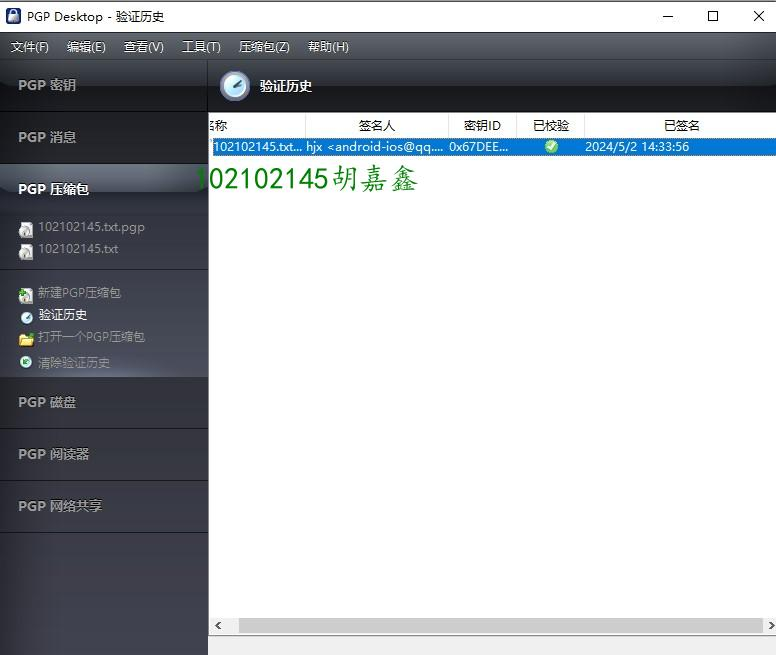
\includegraphics[width=0.45\textwidth]{1_18.jpg}
  \end{center}
\end{figure}

解密结果.
\begin{figure}[H]
  \begin{center}
    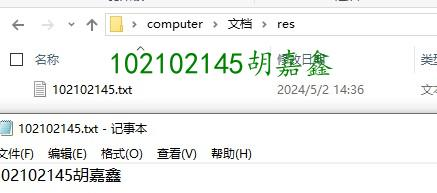
\includegraphics[width=0.45\textwidth]{1_19.jpg}
  \end{center}
\end{figure}

文件签名.
\begin{figure}[H]
  \begin{center}
    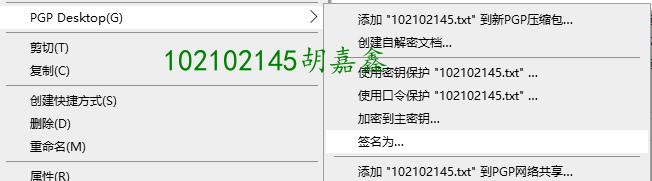
\includegraphics[width=0.45\textwidth]{1_20.jpg}
  \end{center}
\end{figure}
\begin{figure}[H]
  \begin{center}
    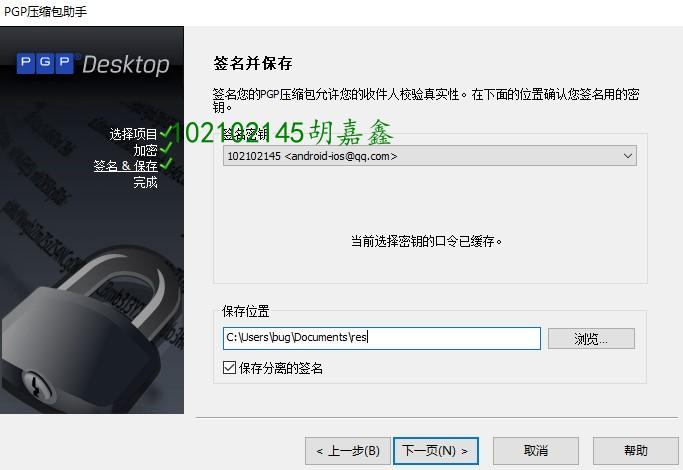
\includegraphics[width=0.45\textwidth]{1_21.jpg}
  \end{center}
\end{figure}

校验结果查看.
\begin{figure}[H]
  \begin{center}
    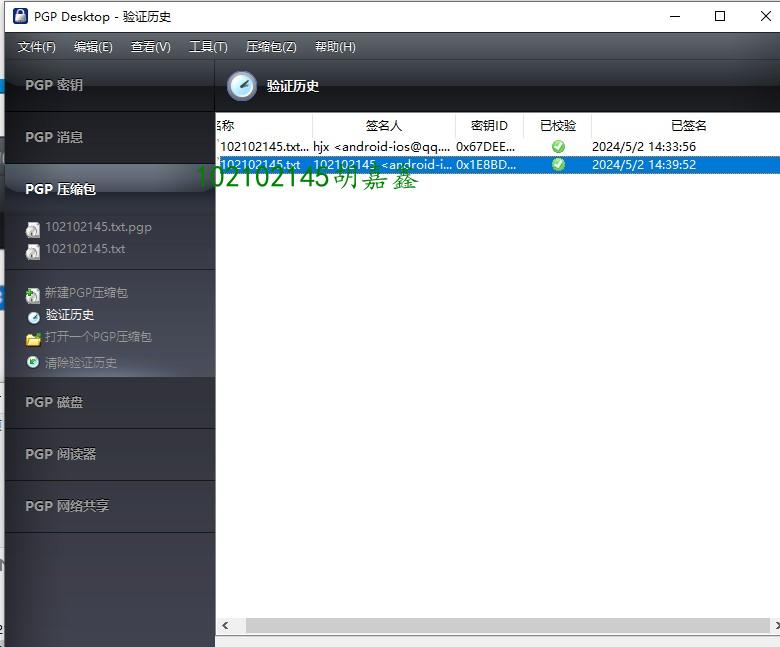
\includegraphics[width=0.45\textwidth]{1_22.jpg}
  \end{center}
\end{figure}
%
\section{Email 的加密与签名}
% 该部分包括使用使用 Web 网页的 email 的书写、剪切、加密剪贴板内容、邮件发送、
% 邮件接收、复制密文邮件、PGP 解密剪贴板内容等步骤。
用邮箱 \texttt{android-ios@qq.com} 发送邮件给
\texttt{1922506058@qq.com},下图是原始信息.
\begin{figure}[H]
  \begin{center}
    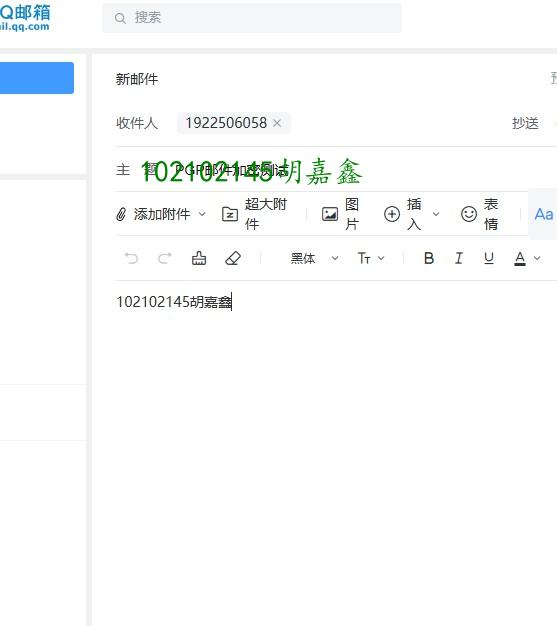
\includegraphics[width=0.45\textwidth]{1_24.jpg}
  \end{center}
\end{figure}

将原始信息复制,用 PGP 剪贴板进行加密.
\begin{figure}[H]
  \begin{center}
    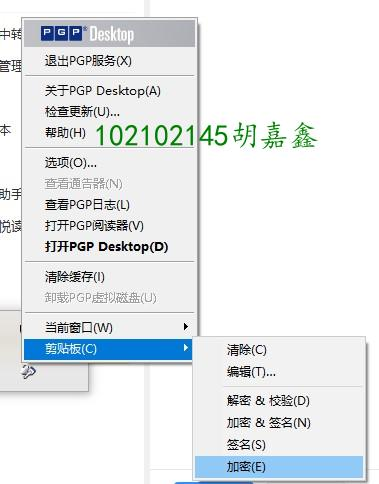
\includegraphics[width=0.45\textwidth]{1_25.jpg}
  \end{center}
\end{figure}

选择用收件人的公钥进行加密.
\begin{figure}[H]
  \begin{center}
    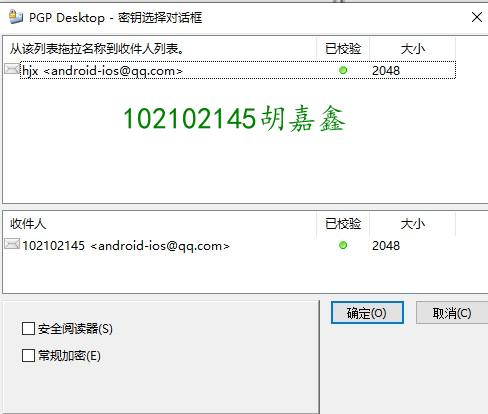
\includegraphics[width=0.45\textwidth]{1_26.jpg}
  \end{center}
\end{figure}

将加密后内容粘贴到发件框中,覆盖原来的未加密内容.
\begin{figure}[H]
  \begin{center}
    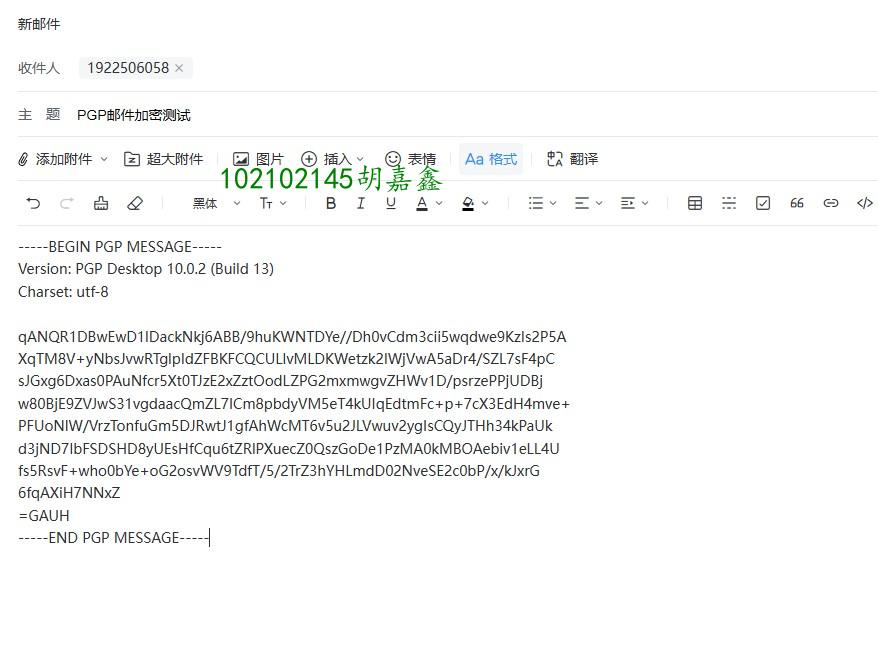
\includegraphics[width=0.45\textwidth]{1_27.jpg}
  \end{center}
\end{figure}

登录接收端账号 \texttt{1922506058@qq.com},复制接收信息到剪贴板.
\begin{figure}[H]
  \begin{center}
    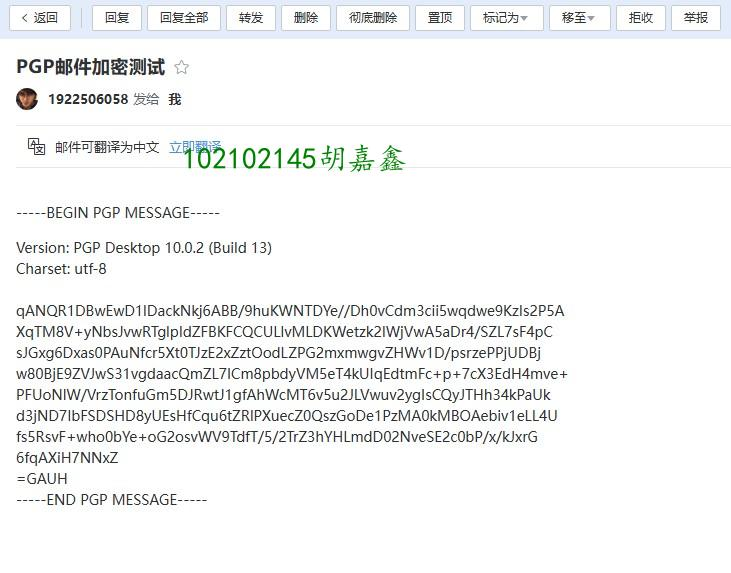
\includegraphics[width=0.45\textwidth]{1_28.jpg}
  \end{center}
\end{figure}

使用接收端私钥进行解密, 解密后还原出原始内容如下:
\begin{figure}[H]
  \begin{center}
    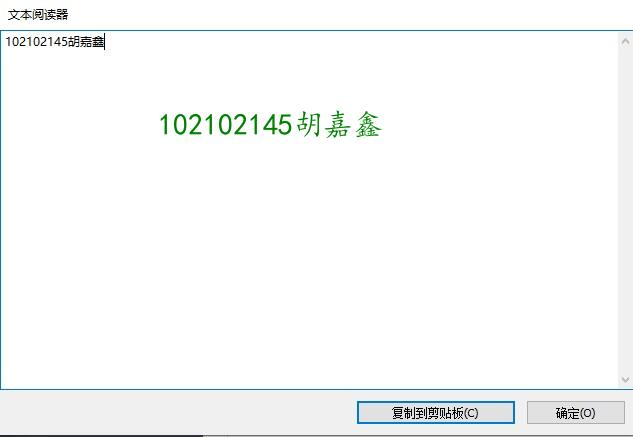
\includegraphics[width=0.45\textwidth]{1_29.jpg}
  \end{center}
\end{figure}

% 加密邮件可以 2 个同学以上合作完成一个实验,分别书写个人通信、操作的部分。
\section{文件的粉碎}
% 该部分包括使用 PGP 软件安全删除粉碎个人的隐私数据文档、文件夹等。
\textbf{相关技术原理}: \\
存储在硬盘中的每个文件都可分为两部分:文件头和存储数据的数据区。

文件头用来记录文件名、文件属性、占用簇号等信息,
文件头保存在一个簇并映射在 FAT 表(文件分配表)中。
而真实的数据则是保存在数据区当中的。平常所做的删除,其实是修改文件头
的前 2 个代码,这种修改映射在 FAT 表中,就为文件作了删除标记,
并将文件所占簇号在 FAT 表中的登记项清零,表示释放空间,这也就是平常删除文件后,硬盘空间增大的原因。

而真正的文件内容仍保存在数据区中,并未得以删除。要等到以后的数据写入,把此数据
区覆盖掉,这样才算是彻底把原来的数据删除。如果不被后来保存的数据覆盖,它就不会
从磁盘上抹掉。用 Fdisk 分区和 Format 格式化和文件的删除类似,前者只是改变了分区
表,后者只是修改了 FAT 表,都没有将数据从数据区直接删除。

由文件删除的原理可知,要彻底删除数据,只有把删除文件所在的数据区完全覆盖掉。
绝大部分彻底删除工具所使用的就是这个道理:把无用的数据反复写入删除文件的数据
区,并进行多次地覆盖,从而达到完全删除文件的目的。

\begin{figure}[H]
  \begin{center}
    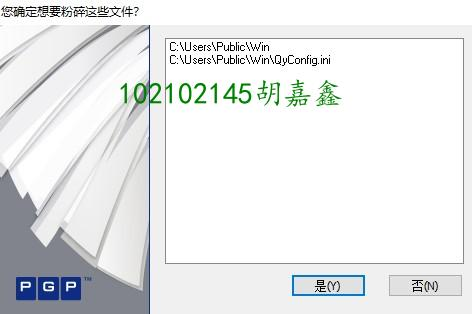
\includegraphics[width=0.45\textwidth]{1_30.jpg}
  \end{center}
\end{figure}
%
\section{虚拟磁盘的加密}
% 该部分包括使用 PGP 创建、加密生成一个加密的虚拟磁盘功能。
\textbf{相关技术原理}: \\
把文件,网络文件,内存等通过技术手段``伪装''成磁盘,让用户感觉像一个真实磁
盘的``磁盘''就称为虚拟磁盘。

\begin{figure}[H]
  \begin{center}
    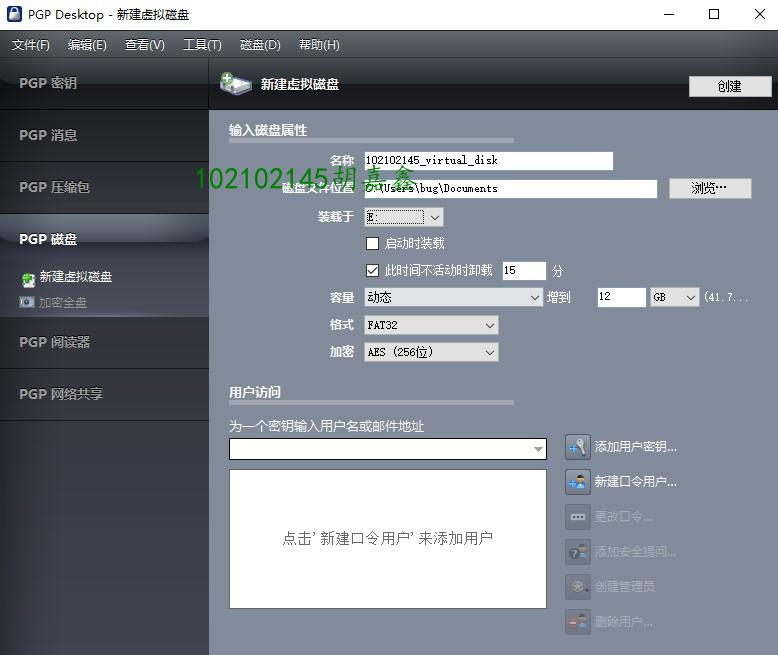
\includegraphics[width=0.45\textwidth]{1_31.jpg}
  \end{center}
\end{figure}
%
\section{磁盘空间的粉碎}
% 该部分包括使用 PGP 右击逻辑磁盘,实现对磁盘已删除内容的彻底清空操作。
原理类似文件的粉碎.
\begin{figure}[H]
  \begin{center}
    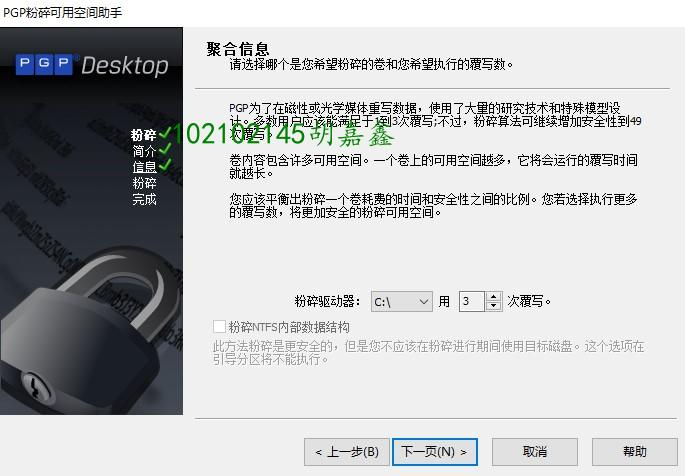
\includegraphics[width=0.45\textwidth]{1_32.jpg}
  \end{center}
\end{figure}
\begin{figure}[H]
  \begin{center}
    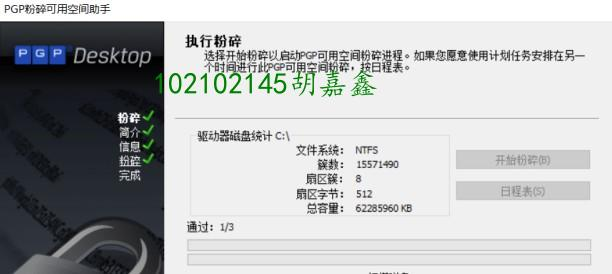
\includegraphics[width=0.45\textwidth]{1_33.jpg}
  \end{center}
\end{figure}
%
\end{document}
